\pagebreak
\section{Aprendizaje Automatizado}
El aprendizaje automatizado es un campo de la ciencia de la computación donde se busca darle a las computadores la habilidad de aprender sin ser explícitamente programadas. El término se le atribuye a \textbf{Arthur Samuel}, un pionero del campo de la inteligencia artificial, quien lo acuñó en 1959 \cite{kohaviProvost}. Algunos autores también señalan al profesor James Townsend de la Universidad de Indiana quien se refiere al término en sus trabajos sobre matrices de confusión \cite{townsend}.

Es interesante que los métodos de aprendizaje automatizado proliferaron de forma paralela al concepto de ciencia de datos, y solo fueron absorbidos por esta en los últimos diez años. Alpaydim nos describe el aprendizaje automatizado como la programación de computadoras para optimizar un criterio de desempeño utilizando datos o experiencia pasada \cite{alpaydin}. Tom Mitchell respeta este concepto al describir el aprendizaje automatizado como "\ldots la construcción de programas computacionales que aprenden con la experiencia\ldots” \cite[pag. XV]{mitchell}. Solo Peter Harrington utiliza una descripción mucho más simplista al determinar que “El aprendizaje automatizado es la extracción de información de la data.” \cite[pag. 5]{harrington}.

Estudiar los procedimientos de aprendizaje automatizado equivale a estudiar tres temas principales que los componen.

\begin{itemize}
	\item Diseño del estudio: conjuntos de entrenamiento y conjuntos de predicción
	\item Problemas conceptuales: error fuera de la muestra, curvas ROC
	\item Implementación práctica: en este caso en particular, un tema que se cubrirá con la biblioteca Caret
\end{itemize}

Todo el mundo predice todo tipo de aseveraciones, desde el resultado de una elección presidencial hasta el partido de fútbol del domingo de una liga en particular. Pero en el sentido estricto de la palabra, ¿qué significa predecir? En nuestro contexto científico, definiremos el acto de predecir como el resultado de utilizar la probabilidad y muestreo para la selección de un conjunto de entrenamiento, el cual utilizaremos para construir las características de diseño de una función de predicción. La función utilizará dichas características para generar nuevas predicciones.  Los componentes para la selección adecuada de variables de predicción son los siguientes:

\begin{figure}[h!]
    \centering
    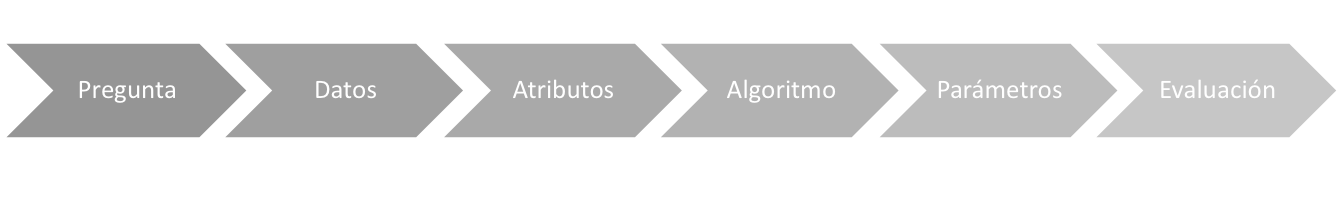
\includegraphics[width = 6 in]{images/esquemaVariablesPrediccion.png}
    \caption{Esquema de Generación de Variables de Predicción}
\end{figure}

Un ejemplo muy común utilizado generalmente para explicar el uso del aprendizaje automatizado es la detección de correo chatarra, también conocido como spam. Podemos utilizar atributos cuantitativos de los mensajes, por ejemplo la frecuencia de ciertas palabras, para que un modelo se entrene y pueda predecir dentro de ciertos rangos de certeza si un correo cualquiera es o no spam.

\subsection{Importancia Relativa de Los Pasos}

Hay una secuencia de pasos importante para la consecución de modelos de aprendizaje automatizado coherentes.

\begin{figure}[h!]
    \centering
    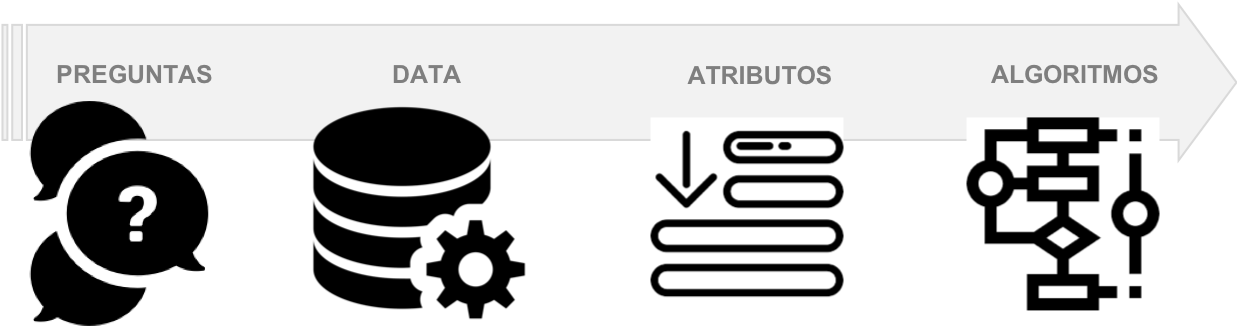
\includegraphics[width = 6 in]{images/pasosAprendizajeAutomatizado.png}
    \caption{Pasos para la Consecución de Modelos con Aprendizaje Automatizado}
\end{figure}

La combinación de algunos datos y un deseo extremo de conseguir una respuesta no nos asegura que una razonable pueda extraerse de un cuerpo cualquiera de información \cite{tukey}. También es útil recordar que la calidad de los datos que ingresan al conjunto de entrenamiento tienen un efecto sobre el resultado del modelo. Datos que no son útiles no aportan nada. Es mucho mejor que la data sea curada y organizada de manera que tenga alta relevancia al tema de estudio.

Los buenos atributos son aquellos que comparten las siguientes características:

\begin{enumerate}
	\item ayudan a comprimir la data
	\item retienen el mayor volumen de información relevante
	\item son creados basados en un modelo experto del modelo a aplicarse
\end{enumerate}

No es fácil hacer una buena selección de atributos que mas adelante se convertirán en variables de predicción. Los errores mas comunes son los siguientes.

\begin{enumerate}
	\item tratar de automatizar la selección de atributos
	\item no prestar la atención necesaria a las variaciones y particularidades de los datos
	\item desechar información importante innecesariamente
\end{enumerate}

En este sentido los algoritmos importan mucho menos que la selección y curación de la data a utilizar. Los mejores métodos de aprendizaje automatizado reúnen una serie de características que los hace justamente sobresalir del montón. Las características en mención son las siguientes:

\begin{enumerate}
	\item Interpretable: el modelo debe ser capaz de llegar a una solución que pueda entenderse y aplicarse al problema que se tiene a mano.
	\item Simples: el modelo debe ser lo suficientemente sencillo para implementarse en un ambiente científico real con las herramientas disponibles.
	\item Precisos: el modelo debe tener un nivel mínimo de precisión que esté en linea con los parámetros esperados por la investigación científica tradicional.
	\item Rápidos (de entrenar y evaluar): el modelo debe ser capaz de ser entrenado y evaluado dentro de marcos normales de tiempo y recursos. \item Escalables: el modelo, de ser posible, debe ser capaz de escalar e implementarse en sistemas de menor costo de recursos.
\end{enumerate}

La predicción de modelos se basa mucho en el arte de compensar beneficios versus necesidades.

\begin{enumerate}
	\item interpretación de los datos vs. precisión
	\item velocidad vs. precisión
	\item simplicidad vs. precisión
	\item modelos escalables vs. precisión
\end{enumerate}

A pesar de tener que sopesar la mejor forma de compensar todas estas variables, la interpretación es muy importante y debe conservar su lugar, ya que poco sirve un modelo rápido y preciso que no se puede interpretar. Muchos autores otorgan un segundo lugar de importancia a lo escalable del modelo. Se han dado casos donde modelos muy precisos no se han podido poner en producción por la complejidad de escalar el algoritmo. El caso mas mencionado es el premio NETFLIX, el cual otorgo un millón de dolares al equipo con el mejor modelo de predicción de gustos de sus clientes, solo para luego llegar a la conclusión que el mismo era demasiado complejo y lento de escalar en producción y archivarlo \cite{techdirt}.

\subsection{Métodos Supervisados y No-Supervisados}
Para los autores Hastie, Tibshirani, y Friedman el aprendizaje supervisado intenta aprender una función f de predicción a través del uso de uso juegos de datos de entrenamiento en forma de muestras del total de los datos disponibles. El uso de datos de entrenamiento le permite al sistema aprender y minimizar el error del modelo de predicción \cite{theElements}.

Harrington nos da una explicación más sencilla del término, al aclarar que el aprendizaje supervisado es aquel que le pide al computador aprender de los datos utilizando una variable específica como objetivo. Esto reduce la complejidad de algoritmos y patrones que se deben derivar de la muestra de datos \cite{harrington}.

El profesor Alpaydin agrega que el aprendizaje supervisado tiene como objeto aprender un mapeo de los elementos de entrada a los de salida, teniendo en cuenta que los valores correctos de estos últimos están dados por el supervisor \cite{alpaydin}.

\subsection{Error Muestral y Error Fuera de Muestra}
El siguiente concepto es fundamental dentro de la teoría de aprendizaje automatizado, y la terminología puede diferir un poco de los términos establecidos en la estadística inferencial.

	\begin{itemize}
		\item \textbf{Error dentro de la muestra:} es el margen de error que se obtiene al utilizar el juego de datos de entrenamiento en la construcción del modelo de predicción. También se conoce como error de re-substitución
		\item  \textbf{Error fuera de muestra:} es el margen de error que se obtiene cuando se aplica el modelo de predicción a un nuevo juego de datos. También se lo conoce como error de generalización.
	\end{itemize}


En este punto debemos aclarar cuales son las ideas principales en las que hay que enfocarse.

\begin{enumerate}
	\item Principalmente estamos interesados mucho mas en el error de generalización - el que se obtiene al aplicar un nuevo juego de datos al modelo de predicción - que del margen de error de resubstitución.
	\item El error de resubstitución siempre va a ser menor que el error de generalización
	\item La razón por la cual se da este fenómeno (que el error de resubstitución sea menor que el error de generalización) es el efecto de sobreajuste. El algoritmo se está ajustando de más a los datos.
\end{enumerate}

La data en la ciencia de datos tiene dos partes: señal y ruido. El objetivo del modelo de predicción es el de predecir la señal. Siempre se puede diseñar un modelo perfecto que capture tanto la señal como el ruido. Pero dicho modelo no se desempeñará bien en juegos de datos nuevos.

El efecto de sobreajuste se como la creación de un modelo optimista a partir del juego de datos de entrenamiento. Los métodos que utilizamos buscan interpretar los datos de tal manera que no solo se ajustan a la señal sino al ruido de los mismos. Por esa razón el margen de error de resubstitución (error dentro de la muestra) es tan bajo pero cuando se prueba el mismo modelo entrenado en un juego de datos externo el margen de error generalizado (fuera de la muestra) crece. Se ha comprobado que los errores por sobreajuste ocurren más en modelos complejos que en modelos sencillos. La razón es que muchas veces el modelo complejo es precisamente más complicado para ajustarse mejor a la señal de los datos, sin que estos ajustes sean necesarios - o precisos - al momento de cambiar del juego de datos.

\subsection{Diseño de un Estudio de Aprendizaje Automatizado}
El diseño de una investigación de ciencia de datos tiene seis pasos. El diseño del estudio de un problema de aprendizaje automatizado debe verse como el diseño de la fase de modelo (paso tres) mucho más detallado para no confundirlos. La metodología recomendada por el Dr. Jeff Leek \cite{leek} recomienda los siguientes seis:

\begin{enumerate}
	\item Definir el margen de error deseado
	\item Dividir la data en juegos específicos de entrenamiento, evaluación y validación (opcional)
	\item En el juego de entrenamiento, seleccionar atributos y utilizar validación cruzada
	\item En el juego de entrenamiento, seleccionar la función de predicción; utilizar nuevamente validación cruzada
	\item si no se utilizo validación cruzada, aplicar prueba $1X$ al juego de evaluación
	\item si se utilizo validación cruzada, aplicar prueba al juego de evaluación, refinar el algoritmo, y luego volver a someter $1X$ al juego de validación
\end{enumerate}

A pesar de que no tiene una comprobación científica, la comunidad siempre aconseja evitar las muestras pequeñas de la misma forma que se evitan en la estadística clásica. Una pregunta válida es cuanto de los datos disponibles se deben destinar al juego de entrenamiento, cuantos al juego de validación y cuantos al juego de evaluación. Zumel y Mount \cite{zumelMount} consideran un modelo sencillo de división con 90\% de los datos destinados al entrenamiento de modelos y el 10\% restante a la evaluación. Sin embargo Leek \cite{leek} en su libro \emph{Data Style} nos da un juego de reglas mas comprensivas de como distribuir los datos según el volumen de los mismos.

\textbf{A. Si el volumen de datos es grande}
\begin{itemize}
	\item 60\% para el juego de entrenamiento
	\item 20\% para el juego de evaluación
	\item 20\% para el juego de validación
\end{itemize}

\textbf{B. Si el volumen de datos es mediano}
\begin{itemize}
	\item 60\% para el juego de entrenamiento
	\item 40\% para el juego de evaluación
\end{itemize}

\textbf{C. Si el volumen de datos es pequeño}
\begin{itemize}
	\item entrenar sobre el 100\% de los datos
	\item utilizar validación cruzada sobre el mismo juego que se entrenó
	\item no ocultar el hecho hacer alusión en la investigación de la muestra poco representativa
\end{itemize}

La tentación de utilizar el juego de datos de validación y/o evaluación es muy grande para todos los científicos de datos noveles. Sin embargo la literatura concuerda en que no se debe utilizar la evaluación sino hacia el final del proceso.

La selección de que datos en particular deben elegirse en cada grupo debe ser aleatoria, con un porcentaje definido en cada uno pero total certeza de que no hay parcialidad en la selección. En el caso del lenguaje R, la biblioteca CARET tiene incorporada funciones para garantizar asignaciones de datos a los grupos de entrenamiento y evaluación totalmente aleatorios. Los juegos finales de datos deben reflejar sin embargo las mismas estructuras del problema. Un claro ejemplo son las series de tiempo \cite{hyndman} en las cuales los datos tiene un componente de tiempo que denota un orden en especial. De estos grupos debe seleccionarse muestras aleatorias pero representativas de los periodos de tiempo a fin de tener sentido. A su vez cada sub-muestra debe reflejar el mayor grado de diversidad posible. Esto se debe lograr con selección aleatoria pero a veces es difícil mantener dicho balance con la mezcla posible de atributos.

\subsection{Tipo de Errores}
El concepto de error en estadística es uno que embarca varias dimensiones. En lo que respecta al aprendizaje automatizado, no importa que tan grande sea la muestra ni que tan exacto sea el algoritmo, siempre cabe la probabilidad - aunque pequeña - que una predicción sea falsa a pesar de que arroja un resultado positivo. Podemos entonces dividir los tipos de errores según su predicción y verdadera naturaleza \cite{yakir}.

En lineas generales diremos que un resultado es positivo si ha sido identificado como tal, y que es negativo si ha sido rechazado. De tal forma:
\begin{itemize}
	\item \textbf{verdadero positivo:} es aquel que ha sido correctamente identificado
	\item \textbf{falso positivo:} es aquel que ha sido incorrectamente identificado
	\item \textbf{verdadero negativo:} es aquel que ha sido correctamente rechazado
	\item \textbf{falso negativo:} es aquel que ha sido incorrectamente rechazado
\end{itemize}

La combinación de los siguientes resultados nos permite medir estadísticamente variables pertinentes a los resultados del modelo. Estas variables se conocen como sensibilidad, especificidad, valor predictivo positivo, valor predictivo negativo, y exactitud.

\textbf{Sensibilidad:} La sensibilidad es la probabilidad que un fenómeno arroje un valor positivo cuando realmente lo es. Por ejemplo, un examen de una enfermedad da positivo cuando el paciente realmente esta enfermo de dicho padecer. Podemos expresar la formula como un cociente de la siguiente forma:

\begin{equation}
sensibilidad = \frac{VP}{(VP + FN)}
\end{equation}

\textbf{Especificidad:} La especificidad es la probabilidad que un fenómeno arroje un valor negativo cuando realmente no se encuentra presente (o sea es una predicción negativa cuando la realidad también es negativo). Por ejemplo, un examen de embarazo que da negativo cuando la paciente no esta embarazada. Podemos expresar la formula como un cociente de la siguiente forma:

\begin{equation}
especificidad= \frac{VN}{(FP + VN)}
\end{equation}

\textbf{Valor Predictivo Positivo:} El valor predictivo positivo es la probabilidad de que un fenomeno este presente cuando la predicción arroja un valor positivo. Por ejemplo, la probabilidad de que un paciente tenga diabetes cuando el examen arroja positivo. Podemos expresar la formula como un cociente de la siguiente forma:

\begin{equation}
\mbox{\textit{valor predictivo positivo}} = \frac{VP}{(VP + FP)}
\end{equation}

\textbf{Valor Predictivo Negativo:} Lo opuesto del valor predictivo positivo, es la probabilidad de que una prediccion arroje negativo cuando el fenómeno no este presente. Por ejemplo, la probabilidad de que un paciente no se le detecte diabetes cuando en la vida real no la tiene. Podemos expresar la formula como un cociente de la siguiente forma:

\begin{equation}
\mbox{\textit{valor predictivo negativo}} = \frac{VN}{(VN + FN)}
\end{equation}

\textbf{Exactitud:} Quizás el mas sencillo de percibir de forma natural, la exactitud es simplemente la probabilidad de una prediccion correcta. Podemos expresar la formula como un cociente de la siguiente forma:

\begin{equation}
exactitud = \frac{VP + VN}{(VP + FP + VN + FN)}
\end{equation}

\subsubsection{Midiendo Error en Data Continua}
Para data continua, de naturaleza numérico, las dos formas de medir el error mas comunes en aprendizaje automatizado son el error cuadrático medio y la raíz error cuadrático medio.

La raíz error cuadrático media es utilizada con frecuencia para medir la diferencia entre valores (de una muestra y valores de una población) predicha por un modelo o un estimador y los datos observados en la realidad. Este valor representa la desviación estándar de la muestra entre los valores predecidos y los valores observados. Las diferencias individuales entre estas dos medidas se conocen como residuos si son extraídos de la muestra, y errores de predicción si son calculados fuera de muestra.

\begin{equation}
\sqrt{\frac{1}{n}\sum_{i=1}^n(prediccion_{i} - observado_{i})^{2}}
\end{equation}

\subsection{Sobreajuste}
En aprendizaje automatizado, el sobreajuste (también es frecuente emplear el término en inglés overfitting) es el efecto de sobre-entrenar un algoritmo de aprendizaje con unos ciertos datos para los que se conoce el resultado deseado. Daroczi define el sobreajuste como la descripción del modelo en conjunto con el ruido aleatorio de la muestra en vez de solo el fenómeno generador de datos \cite{daroczi}. El sobreajuste ocurre, por ejemplo, cuando el modelo tiene más predictores de los que puede acomodar la muestra de datos.

Según Zumel y Mount, una de las señales de sobreajuste más sencillas de detectar se da cuando un modelo tiene un excelente desempeño en el juego de datos que se entrenó, pero uno muy malo en un juego de datos nuevo \cite{zumelMount}. Esto es causa y efecto de memorizar la data de entrenamiento en vez de aprender reglas generales de la generación del patrón.

\subsection{R y la Biblioteca CARET}
La biblioteca \emph{CARET} (nombre extraído de Classification And Regression Training) es una libreria de funciones en R para optimizar el proceso de crear modelos predictivos. El paquete contiene herramientas para:

\begin{itemize}
	\item segmentar juegos de datos
	\item preproceso de los datos
	\item seleccion de predictores
	\item optimizacion del modelo utilizando reconfiguracion de muestras
	\item estimacion de la importancia de la variable
\end{itemize}

El paquete esta mantenido en GitHub bajo la administración del Doctor en Estadística Max Kuhn \cite{caret}.
